\newcommand{\imageWithGrid}[3]{%
  \begin{tikzpicture}
    \node[anchor=south west,inner sep=0] (image) at (0,0) {\includegraphics[width=#2, height=#3]{#1}};
    \begin{scope}[x={(image.south east)},y={(image.north west)}]
        \foreach \i in {1,...,4} {
            \draw[lightgray,thin] (\i/5,0) -- (\i/5,1); % Vertical lines
            \draw[lightgray,thin] (0,\i/5) -- (1,\i/5); % Horizontal lines
        }
        \draw[black] (0,0) rectangle (1,1);
    \end{scope}
  \end{tikzpicture}%
}


\begin{figure}[t!]
\centering

\tabcolsep=0.04cm
\renewcommand{\arraystretch}{0.8}
\begin{tabular}{ccccc}
    \raisebox{0.5\height}{
        \resizebox{0.05\textwidth}{!}{
        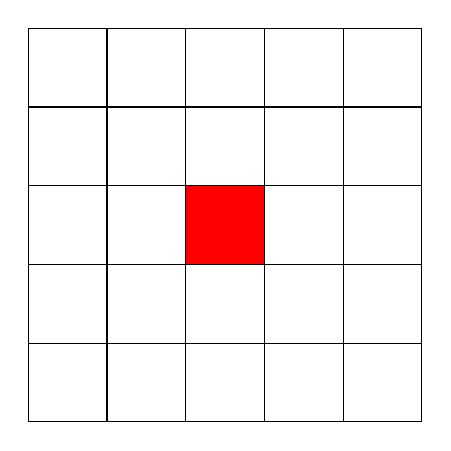
\begin{tikzpicture}
            \foreach \x in {0,1,2,3,4} {
                \foreach \y in {0,1,2,3,4} {
                    \draw[black, thin] (\x,\y) rectangle (\x+1,\y+1);
                }
            }
            \draw[black] (0,0) rectangle (5,5);
            \fill[red] (2,2) rectangle (3,3);
        \end{tikzpicture}}
    } &
    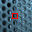
\includegraphics[width=0.09\textwidth]{img/qual/Perforated_Metal_3/LR.annotated.png} &
    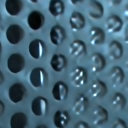
\includegraphics[width=0.09\textwidth]{img/qual/Perforated_Metal_3/EPIT/SR.png} &
    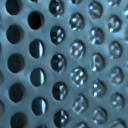
\includegraphics[width=0.09\textwidth]{img/qual/Perforated_Metal_3/SAT/SR.png} &
    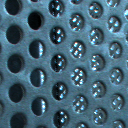
\includegraphics[width=0.09\textwidth]{img/qual/Perforated_Metal_3/HR.png} \\
    \footnotesize{\makecell{SAI\\Location}} & \footnotesize LR & \footnotesize EPIT & \footnotesize M2MT-Net & \footnotesize HR
\end{tabular} \\

(a) SAI location and patch images. \\
\hspace{0pt}

\tabcolsep=0.1cm
\begin{tabular}{cc}
    \imageWithGrid{img/qual/Perforated_Metal_3/EPIT/LAM.png}{0.18\textwidth}{0.18\textwidth} &
    \imageWithGrid{img/qual/Perforated_Metal_3/SAT/LAM.png}{0.18\textwidth}{0.18\textwidth} \\
    % 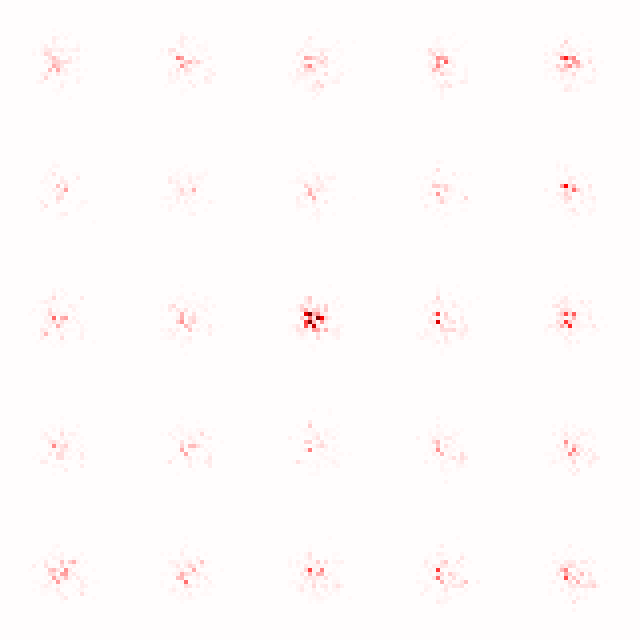
\includegraphics[width=0.22\textwidth,cfbox=black 0.5pt 0pt]{img/qual/Perforated_Metal_3/EPIT/LAM.png} &
    % 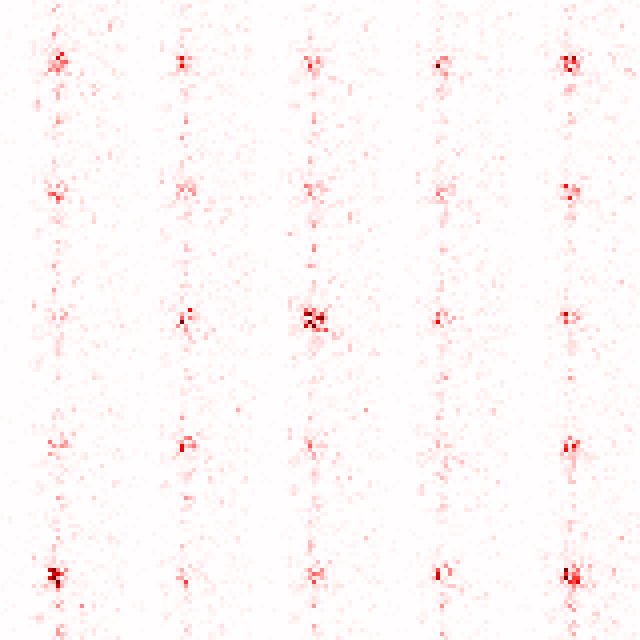
\includegraphics[width=0.22\textwidth,cfbox=black 0.5pt 0pt]{img/qual/Perforated_Metal_3/SAT/LAM.png} \\
    EPIT (DI: 5.9518) & M2MT (DI: 27.2578) \\
\end{tabular} \\
\vspace{8pt}
(b) Local attribution maps of SAIs: Diffusion Index (DI) quantifies the extent of influential pixels.\\
% From the original paper: The Diffusion Index (DI) reflects the range of involved pixels. A higher DI represents a wider range of attention.
%DI represents Diffusion Index.\\
\hspace{0pt}
\caption{Super-resolved results and local attribute maps (LAM) of the proposed M2MT-Net against the current state-of-the-art methods on the \textit{Perforated\_metal\_3} sample.}
% \caption{Illustration of super-resolved images and LAM comparing EPIT and M2MT on a patch of the \textit{Perforated metal 3} sample.}

\label{fig:First}
\end{figure}
